% !TeX root = skripta-konstitutivni-vztahy.tex
% !TeX lastmodified = 2018-10-09

\subsection{Komplexní modul pružnosti viskoelastické látky}
Obecně se jedná výhradně o~modul pružnosti ve smyku $G$, příp. objemový modul pružnosti $K$.
Pro modul pružnosti v~tahu $E$ lze použít jedině v~případě jednodimenzionálního problému, nelze pak aplikovat na víceosou napjatost. 

Závislost mezi napětím a~přetvořením je ovlivněna rychlostí (frekvencí) zatěžování, tedy na ní závisí i~moduly pružnosti.
Pro modul pružnosti ve smyku tedy platí:
\begin{equation}
	G(\omega) = \frac{\sigma(\omega t)}{\varepsilon(\omega t)}
\end{equation}

Pro silové zatěžování (Maxwellův model) s~harmonickým průběhem napětí, který vyjádříme pomocí komplexních čísel, platí:
\begin{equation}
	\sigma(\omega t) = \sigma_a \left[\cos(\omega t) + i \sin(\omega t)\right] = \sigma_a \exp(i \omega t)
\end{equation}

Protože deformace se zpožďuje za napětím, je deformační odezva popsána vztahem:
\begin{equation}
	\varepsilon(\omega t) = \varepsilon_a \left[\cos(\omega t - \delta) + i \sin(\omega t - \delta)\right] = \varepsilon_a \exp[i (\omega t - \delta)]
\end{equation}

\subsubsection{Složky komplexního modulu pružnosti viskoelastické látky}
Dosazením exponenciálních tvarů komplexních vyjádření napětí a~přetvoření do vztahu pro modul pružnosti ve smyku dostaneme:
\begin{equation}
	G(\omega)
	= \frac{\sigma_a \exp(i \omega t)}{\varepsilon \exp\left[i(\omega t - \delta)\right]}
	= \frac{\sigma_a}{\varepsilon_a} \exp\left[i \delta(\omega)\right]
	= G_a \exp\left[i \delta(\omega)\right]
\end{equation}

Exponenciální tvar komplexního modulu můžeme pak převést zpět na tvar goniometrický:
\begin{equation}
	G(\omega)
	= G_a \left\{ \cos\left[\delta(\omega)\right] + i \sin\left[\delta(\omega)\right] \right\}
	= G_\text{Re}(\omega) + i G_\text{Im}(\omega)
	= G'(\omega) + i G''(\omega)
\end{equation}
kde
\begin{description}
	\item[$G_\text{Re}=G'$] je složka ve fázi, odpovídající elastickému chování materiálu, tedy elastický modul,
	\item[$G_\text{Im}=G''$] je složka mimo fázi, odpovídající viskóznímu chování materiálu, tedy ztrátový modul (\textit{loss modulus}).
\end{description}

Komplexní modul je závislý na frekvenci zatěžování; jeho amplituda udává poměr amplitud napětí a~deformace a~fázový úhel definuje fázový posuv mezi napětím a deformací.

\subsubsection{Komplexní modul pružnosti pro deformační zatěžování}
K~analogickému výsledku dospějeme i~pro deformační zatěžování (Voigtův model) s~harmonickým průběhem přetvoření:
\begin{equation}
	\varepsilon(\omega t) = \varepsilon_a \left[\cos(\omega t) + i \sin(\omega t)\right] = \varepsilon_a \exp(i \omega t)
\end{equation}

Napětí se předbíhá před deformací o~fázový posuv $\delta$, takže průběh napětí je popsán rovnicí:
\begin{equation}
	\sigma(\omega t) = \sigma_a \left[\cos(\omega t - \delta) + i \sin(\omega t - \delta)\right] = \sigma_a \exp[i (\omega t - \delta)]
\end{equation}

takže dospějeme ke stejnému vyjádření komplexního modulu pružnosti
\begin{equation}
	G(\omega)
	= \frac{\sigma(\omega t)}{\varepsilon(\omega t)}
	= \frac{\sigma_a \exp\left[ i (\omega t + \delta) \right]}{\varepsilon_a \exp\left( i \omega t \right)}
	= \frac{\sigma_a}{\varepsilon_a} \exp\left[i \delta(\omega) \right]
	= G_a \left[ \cos(\delta) + i \sin(\delta) \right]
\end{equation}

Tangenta fázového posuvu $\delta$ je mírou disipace energie při deformaci materiálu a~nazývá se \texttt{ztrátový faktor}.

\subsubsection{Složky komplexního modulu pružnosti pro jednoduché modely}
Maxwellův model:
\begin{equation}
	G_a = \frac{1}{\sqrt{\frac{1}{G_2} + \frac{1}{\eta^2 \omega^2}}}
	\qquad
	\tan(\delta) = \frac{G}{\eta \omega}
\end{equation}
S~rostoucí frekvencí zatěžování fázový úhel (i~ztrátový faktor) klesá.

Voigtův model:
\begin{equation}
	G_a = \sqrt{G^2 + \eta^2 \omega^2}
	\qquad
	\tan(\delta) = \frac{\eta \omega}{G}
\end{equation}
S~rostoucí frekvencí zatěžování fázový úhel (i~ztrátový faktor) roste.

Kelvinův model:
\begin{equation}
	G_a = G_0 \sqrt{\frac{1 + \omega^2 \tau_\sigma^2}{1 + \omega^2 \tau_\varepsilon^2}}
	\qquad
	\tan(\delta) = \frac{\omega (\tau_\sigma - \tau_\varepsilon)}{1 + \omega^2 \tau_\sigma \tau_\varepsilon}
\end{equation}
Závislost fázového úhlu (ztrátového faktoru) na frekvenci vykazuje lokální extrém (viz dále).

Ve všech případech amplituda komplexního modulu pružnosti roste s~rostoucí frekvencí zatěžování, tedy \textbf{materiál se vždy při rychlejším zatěžování jeví jako tužší}.

\subsubsection{Určení složek komplexního modulu pružnosti v~Kelvinově modelu}
\begin{equation}
	G(\omega)
	= \frac{\sigma(\omega t)}{\varepsilon(\omega t)}
	= G_0 \frac{1 + \omega^2 \tau_{12}\sigma \tau_{12}\varepsilon + i \omega (\tau_\sigma - \tau_\varepsilon)}{1 + \omega^2 \tau_\varepsilon^2}
\end{equation}
\begin{equation}
	G_a(\omega)
	= G_0 \sqrt{\frac{1 + \omega^2 \tau_\sigma^2}{1 + \omega^2 \tau_\varepsilon^2}}
	\qquad
	\tan\left[\delta(\omega)\right]
	= \frac{\omega (\tau_\sigma - \tau_\varepsilon)}{1 + \omega^2 \tau_\sigma \tau_\varepsilon}
\end{equation}

Zvolené parametry modelu jsou $G_0 = \SI{200}{\mega\pascal}, \tau_\sigma = \SI{3}{\second}, \tau_\varepsilon = \SI{2}{\second}$.
\begin{figure}[H]
	\centering
	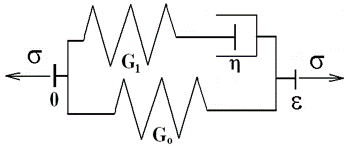
\includegraphics[height=3cm]{kelvinuv-model}
	\caption{Kelvinův model}
	\label{fig:kelvinuv-model}
\end{figure}
Pro tyto parametry ($\eta$ a~$G_1$ jsou zadány nepřímo pomocí časových konstant) jsou dále vykresleny závislosti amplitudy komplexního modulu pružnosti $G_a$ a~ztrátového faktoru $\tan(\delta)$ (vykazuje extrém pro $\omega_\text{ex} = \SI{0.408}{\radian\per\second}$) na úhlové frekvenci zatěžování $\omega$.

Amplituda a~ztrátový faktor komplexního modulu pružnosti jako funkce úhlové frekvence zatěžování v~Kelvinově modelu
\begin{figure}[H]
	\centering
	\begin{minipage}{0.5\linewidth}
		\centering
		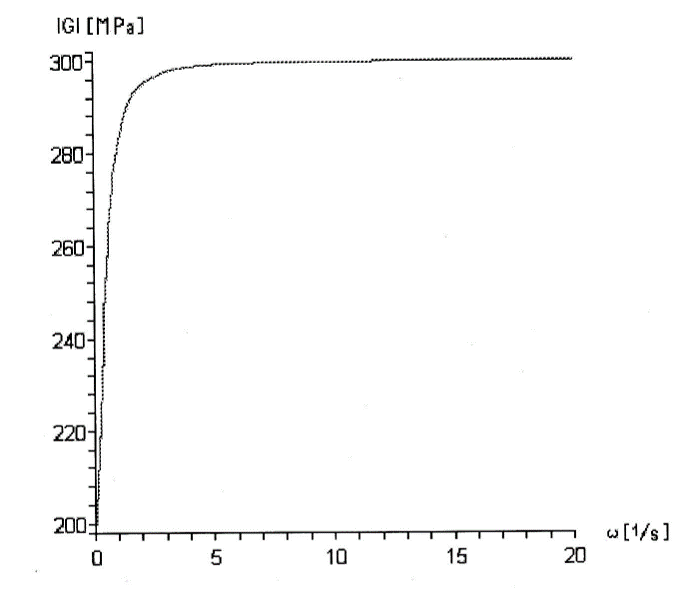
\includegraphics[width=0.5\linewidth]{amplituda-modulu-pruznosti}
		\caption{Amplituda modulu pružnosti}
		\label{fig:amplituda-modulu-pruznosti}
	\end{minipage}%
	\begin{minipage}{0.5\linewidth}
		\centering
		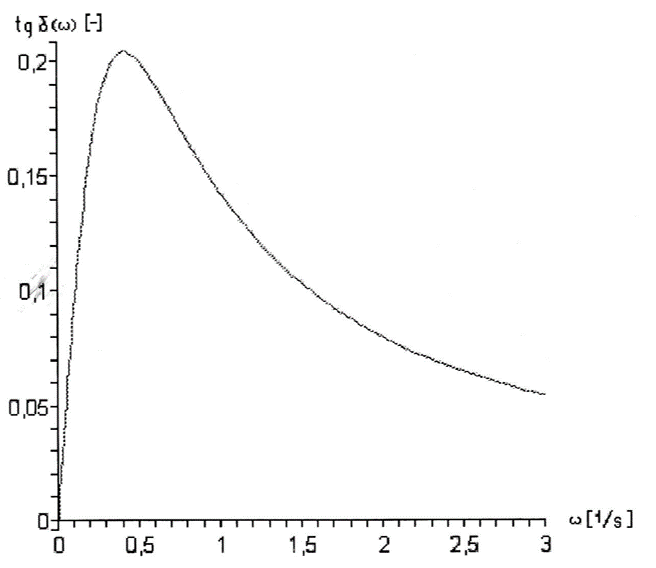
\includegraphics[width=0.5\linewidth]{ztratovy-faktor}
		\caption{Ztrátový faktor}
		\label{fig:ztratovy-faktor}
	\end{minipage}
\end{figure}
